\documentclass{ieeeaccess}
%DIF LATEXDIFF DIFFERENCE FILE
%DIF DEL v1_access.tex   Sat Dec 21 11:26:51 2024
%DIF ADD access.tex      Tue Jan 21 22:21:04 2025
\usepackage{cite}
\usepackage{amsmath,amssymb,amsfonts}
\usepackage{algorithmic}
\usepackage{graphicx}
\usepackage{textcomp}

\usepackage[ruled,noend,linesnumbered]{algorithm2e}
\usepackage{graphicx,color,psfrag}
\usepackage{amsmath}
\usepackage{amsfonts}
\usepackage{amssymb}
\usepackage{bigdelim}
\usepackage{dsfont}
\usepackage{color, soul}
\usepackage{caption}
\usepackage{subcaption}
\usepackage{url}

\def\BibTeX{{\rm B\kern-.05em{\sc i\kern-.025em b}\kern-.08em
    T\kern-.1667em\lower.7ex\hbox{E}\kern-.125emX}}
%DIF PREAMBLE EXTENSION ADDED BY LATEXDIFF
%DIF CFONT PREAMBLE %DIF PREAMBLE
\RequirePackage{color}\definecolor{RED}{rgb}{1,0,0}\definecolor{BLUE}{rgb}{0,0,1} %DIF PREAMBLE
\DeclareOldFontCommand{\sf}{\normalfont\sffamily}{\mathsf} %DIF PREAMBLE
\providecommand{\DIFadd}[1]{{\protect\color{blue} \sf #1}} %DIF PREAMBLE
\providecommand{\DIFdel}[1]{{\protect\color{red} \scriptsize #1}} %DIF PREAMBLE
%DIF SAFE PREAMBLE %DIF PREAMBLE
\providecommand{\DIFaddbegin}{} %DIF PREAMBLE
\providecommand{\DIFaddend}{} %DIF PREAMBLE
\providecommand{\DIFdelbegin}{} %DIF PREAMBLE
\providecommand{\DIFdelend}{} %DIF PREAMBLE
%DIF FLOATSAFE PREAMBLE %DIF PREAMBLE
\providecommand{\DIFaddFL}[1]{\DIFadd{#1}} %DIF PREAMBLE
\providecommand{\DIFdelFL}[1]{\DIFdel{#1}} %DIF PREAMBLE
\providecommand{\DIFaddbeginFL}{} %DIF PREAMBLE
\providecommand{\DIFaddendFL}{} %DIF PREAMBLE
\providecommand{\DIFdelbeginFL}{} %DIF PREAMBLE
\providecommand{\DIFdelendFL}{} %DIF PREAMBLE
\newcommand{\DIFscaledelfig}{0.5}
%DIF HIGHLIGHTGRAPHICS PREAMBLE %DIF PREAMBLE
\RequirePackage{settobox} %DIF PREAMBLE
\RequirePackage{letltxmacro} %DIF PREAMBLE
\newsavebox{\DIFdelgraphicsbox} %DIF PREAMBLE
\newlength{\DIFdelgraphicswidth} %DIF PREAMBLE
\newlength{\DIFdelgraphicsheight} %DIF PREAMBLE
% store original definition of \includegraphics %DIF PREAMBLE
\LetLtxMacro{\DIFOincludegraphics}{\includegraphics} %DIF PREAMBLE
\newcommand{\DIFaddincludegraphics}[2][]{{\color{blue}\fbox{\DIFOincludegraphics[#1]{#2}}}} %DIF PREAMBLE
\newcommand{\DIFdelincludegraphics}[2][]{% %DIF PREAMBLE
\sbox{\DIFdelgraphicsbox}{\DIFOincludegraphics[#1]{#2}}% %DIF PREAMBLE
\settoboxwidth{\DIFdelgraphicswidth}{\DIFdelgraphicsbox} %DIF PREAMBLE
\settoboxtotalheight{\DIFdelgraphicsheight}{\DIFdelgraphicsbox} %DIF PREAMBLE
\scalebox{\DIFscaledelfig}{% %DIF PREAMBLE
\parbox[b]{\DIFdelgraphicswidth}{\usebox{\DIFdelgraphicsbox}\\[-\baselineskip] \rule{\DIFdelgraphicswidth}{0em}}\llap{\resizebox{\DIFdelgraphicswidth}{\DIFdelgraphicsheight}{% %DIF PREAMBLE
\setlength{\unitlength}{\DIFdelgraphicswidth}% %DIF PREAMBLE
\begin{picture}(1,1)% %DIF PREAMBLE
\thicklines\linethickness{2pt} %DIF PREAMBLE
{\color[rgb]{1,0,0}\put(0,0){\framebox(1,1){}}}% %DIF PREAMBLE
{\color[rgb]{1,0,0}\put(0,0){\line( 1,1){1}}}% %DIF PREAMBLE
{\color[rgb]{1,0,0}\put(0,1){\line(1,-1){1}}}% %DIF PREAMBLE
\end{picture}% %DIF PREAMBLE
}\hspace*{3pt}}} %DIF PREAMBLE
} %DIF PREAMBLE
\LetLtxMacro{\DIFOaddbegin}{\DIFaddbegin} %DIF PREAMBLE
\LetLtxMacro{\DIFOaddend}{\DIFaddend} %DIF PREAMBLE
\LetLtxMacro{\DIFOdelbegin}{\DIFdelbegin} %DIF PREAMBLE
\LetLtxMacro{\DIFOdelend}{\DIFdelend} %DIF PREAMBLE
\DeclareRobustCommand{\DIFaddbegin}{\DIFOaddbegin \let\includegraphics\DIFaddincludegraphics} %DIF PREAMBLE
\DeclareRobustCommand{\DIFaddend}{\DIFOaddend \let\includegraphics\DIFOincludegraphics} %DIF PREAMBLE
\DeclareRobustCommand{\DIFdelbegin}{\DIFOdelbegin \let\includegraphics\DIFdelincludegraphics} %DIF PREAMBLE
\DeclareRobustCommand{\DIFdelend}{\DIFOaddend \let\includegraphics\DIFOincludegraphics} %DIF PREAMBLE
\LetLtxMacro{\DIFOaddbeginFL}{\DIFaddbeginFL} %DIF PREAMBLE
\LetLtxMacro{\DIFOaddendFL}{\DIFaddendFL} %DIF PREAMBLE
\LetLtxMacro{\DIFOdelbeginFL}{\DIFdelbeginFL} %DIF PREAMBLE
\LetLtxMacro{\DIFOdelendFL}{\DIFdelendFL} %DIF PREAMBLE
\DeclareRobustCommand{\DIFaddbeginFL}{\DIFOaddbeginFL \let\includegraphics\DIFaddincludegraphics} %DIF PREAMBLE
\DeclareRobustCommand{\DIFaddendFL}{\DIFOaddendFL \let\includegraphics\DIFOincludegraphics} %DIF PREAMBLE
\DeclareRobustCommand{\DIFdelbeginFL}{\DIFOdelbeginFL \let\includegraphics\DIFdelincludegraphics} %DIF PREAMBLE
\DeclareRobustCommand{\DIFdelendFL}{\DIFOaddendFL \let\includegraphics\DIFOincludegraphics} %DIF PREAMBLE
%DIF END PREAMBLE EXTENSION ADDED BY LATEXDIFF

\begin{document}
\history{Date of publication xxxx 00, 0000, date of current version xxxx 00, 0000.}
\doi{10.1109/ACCESS.20xx.0000000}

\title{Visibility Aware In-Hand Object Pose Tracking in Videos with Transformers}

\author{\uppercase{Phan Xuan Tan}\authorrefmark{1},
\uppercase{Dinh-Cuong Hoang}\authorrefmark{2},
\uppercase{Eiji Kamioka}\authorrefmark{1},
\uppercase{Anh-Nhat Nguyen}\authorrefmark{3},
\uppercase{Duc-Thanh Tran}\authorrefmark{3}
\uppercase{Van-Hiep Duong}\authorrefmark{3},
\uppercase{Anh-Truong Mai}\authorrefmark{3},
\uppercase{Duc-Long Pham}\authorrefmark{3},
\uppercase{Khanh-Toan Phan}\authorrefmark{3},
\uppercase{Xuan-Tung Dinh}\authorrefmark{3},
\uppercase{Tran Thi Thuy Trang}\authorrefmark{3},
\uppercase{Xuan-Duong Pham}\authorrefmark{3},
\uppercase{Nhat-Linh Nguyen}\authorrefmark{3},
\uppercase{Thu-Uyen Nguyen}\authorrefmark{3},
\uppercase{Viet-Anh Trinh}\authorrefmark{2},
\uppercase{Khanh-Duong Tran}\authorrefmark{2}, and
\uppercase{Son-Anh Bui}\authorrefmark{2}}

\address[1]{College of Engineering, Shibaura Institute of Technology, Tokyo 135-8548, Japan}
\address[2]{Greenwich Vietnam, FPT University, Hanoi, 10000, Vietnam}
\address[3]{IT Department, FPT University, Hanoi, 10000, Vietnam}

%\tfootnote{This paragraph of the first footnote will contain support
%information, including sponsor and financial support acknowledgment. For
%example, ``This work was supported in part by the U.S. Department of
%Commerce under Grant BS123456.''}

\markboth
{P. X. Tan \headeretal: In-Hand Object Pose Tracking}
{P. X. Tan \headeretal: In-Hand Object Pose Tracking}

\corresp{Corresponding author: Dinh-Cuong Hoang (e-mail: cuonghd12@fe.edu.vn).}


\begin{abstract}

In-hand object pose estimation is essential in various engineering applications, such as quality inspection, reverse engineering, and automated manufacturing processes. However, achieving accurate pose estimation becomes difficult when objects are heavily occluded by the hand or blurred due to motion. To address these challenges, we propose a novel framework that leverages the power of transformers for spatial-temporal reasoning across video sequences. Our approach utilizes transformers to capture both spatial relationships within each frame and temporal dependencies across consecutive frames, allowing the model to aggregate information over time and improve pose predictions. A key innovation of our framework is the introduction of a visibility-aware module, which dynamically adjusts pose estimates based on the object's visibility. This module utilizes temporally-aware features extracted by the transformers, allowing the model to aggregate pose information across multiple frames. By integrating this aggregated information, the model can maintain high accuracy even when portions of the object are not visible in certain frames. This capability is particularly crucial in dynamic environments where the object's appearance can change rapidly due to hand movements or interactions with other objects. Extensive experiments demonstrate that our method significantly outperforms state-of-the-art techniques, achieving a 6\% improvement in overall accuracy and over 11\% better performance in handling occlusions.

\end{abstract}

\begin{keywords}
Pose estimation, robot vision systems , intelligent systems,   deep learning, supervised learning, machine vision.
\end{keywords}

\titlepgskip=-21pt

\maketitle

%%%%%%%%%%%%%%%%%%%%%%%%%%%%%%%%%%%%%%%%%%%%%%%%%%%%%%%%%%%%%%%%%%%%

\section{Introduction}
\label{sec:intro}

Accurate estimation of an object's pose from images is a crucial task with broad applications in engineering, including robotic assembly \DIFdelbegin \DIFdel{\cite{trabelsi2021pose, hoang2023grasp, wang2021gdr, hoang2022context}, manipulation \cite{wang2019densefusion, hoang2024collision, zakharov2019dpod, tan2024attention} }\DIFdelend \DIFaddbegin \DIFadd{, manipulation }\DIFaddend augmented reality-driven design\DIFdelbegin \DIFdel{\cite{billings2019silhonet, hoang2024object, peng2019pvnet, hoang2025attention}}\DIFdelend , and automated quality inspection systems \DIFdelbegin \DIFdel{\cite{marullo20236d, du2021vision, cho2024integration}}\DIFdelend \DIFaddbegin \DIFadd{\cite{trabelsi2021pose, hoang2024object, wang2021gdr}}\DIFaddend . The pose, comprising both rotation and translation, provides essential information about the object's position and orientation relative to the camera, enabling systems to interact with the environment in a meaningful way \DIFdelbegin \DIFdel{\cite{hoang2024graspability, peng2019pvnet, wang2021gdr, hoang2022voting}}\DIFdelend \DIFaddbegin \DIFadd{\cite{hoang2024graspability, peng2019pvnet, wang2021gdr}}\DIFaddend . However, achieving robust and precise pose estimation, especially under challenging conditions such as occlusions and complex backgrounds, remains an open research problem\DIFdelbegin \DIFdel{\cite{marullo20236d, vu2024occlusion, chen2016innovative}}\DIFdelend . 

In-hand object pose estimation, in particular, presents a unique set of challenges. Unlike static or freely moving objects, in-hand objects are often subjected to rapid and complex motions, as well as frequent occlusions caused by the hand itself or other environmental factors \cite{chao2021dexycb, hoang2024multi, garcia2018first, llop2022benchmarking}. These conditions lead to significant variations in the object's appearance from frame to frame, complicating the task of accurately tracking its pose over time. Moreover, the proximity of the object to the camera often results in partial or full occlusions, making it difficult to extract reliable visual cues for pose estimation \DIFdelbegin \DIFdel{\cite{hoang2016sub, wang20216d, li2019cdpn, hoang2020panoptic}}\DIFdelend \DIFaddbegin \DIFadd{\cite{wang20216d, li2019cdpn, hoang2020panoptic}}\DIFaddend . Traditional approaches to pose estimation have largely relied on either single-frame methods or handcrafted features, which often struggle to capture the intricate spatial and temporal dependencies present in dynamic scenes \cite{billings2019silhonet, peng2019pvnet}. These methods are particularly vulnerable to errors when the object is partially or fully occluded, as they lack the necessary context to accurately infer the object's pose in such scenarios \DIFdelbegin \DIFdel{\cite{hoang2019object, trabelsi2021pose, rad2017bb8, hoang2020object}}\DIFdelend \DIFaddbegin \DIFadd{\cite{trabelsi2021pose, rad2017bb8, hoang2020object}}\DIFaddend . Additionally, the occlusions and hand-object interactions inherent to in-hand pose estimation introduce further complexity, demanding more sophisticated models that can leverage temporal information to compensate for the lack of visual evidence in individual frames.

Another research direction emphasizes joint estimation of both hand and object poses. Many of these approaches, such as \DIFdelbegin \DIFdel{\cite{doosti2020hope, lin2023harmonious, wang2023interacting, woo2023survey}}\DIFdelend \DIFaddbegin \DIFadd{\cite{doosti2020hope, lin2023harmonious, wang2023interacting}}\DIFaddend , rely on RGB inputs and utilize parameterized models like MANO \cite{romero2022embodied} model to capture hand articulation. Estimating both hand and object poses presents significant challenges due to the high flexibility of the hand, frequent self-occlusions, and the complex interactions between the hand and the object. These difficulties often result in increased errors, particularly when precise object localization is essential. Additionally, the hand-object interaction introduces complex, non-rigid transformations that are difficult to model effectively. Despite these challenges, joint estimation of hand and object poses is critical in applications like telemedicine and immersive gaming, where synchronized and accurate hand-object interaction is vital. However, in many practical scenarios, such as smart manufacturing \DIFdelbegin \DIFdel{(\cite{son2022past}) }\DIFdelend or augmented reality for design evaluation\DIFdelbegin \DIFdel{\cite{park2015spatial}}\DIFdelend , the primary concern is accurately tracking the object's pose. For example, in package sorting or AR-based product identification, the main focus is on determining the precise orientation and position of the object, which is crucial for tasks like scanning barcodes or overlaying virtual information. In industrial automation, especially in precision machining or robotic assembly, tracking the object's pose often takes precedence over the hand or tool's pose. For instance, in a high-precision CNC machining setup, the focus is on accurately positioning and orienting the workpiece to ensure that the machining process meets tight tolerances. In these cases, simplifying the problem by concentrating solely on object pose estimation results in more efficient and practical solutions, while the hand's pose becomes secondary to the overall task.

In this paper, we propose a novel approach for in-hand object pose estimation in videos, addressing the inherent challenges posed by dynamic hand movements and frequent occlusions. Our method begins by leveraging a pre-trained convolutional neural network (CNN) to extract rich spatial features from each frame of the video sequence. These features serve as the foundational representation of the object, capturing crucial spatial information that is essential for accurate pose estimation. However, single-frame spatial features alone are insufficient for robust pose tracking in complex, real-world scenarios where objects are often partially or fully occluded by the hand or other environmental elements. To overcome this limitation, we incorporate a transformer-based temporal reasoning module that processes the sequence of frames as a coherent temporal entity. The transformers in our model are specifically designed to capture both spatial and temporal dependencies across frames, allowing the network to model the evolution of the object's pose over time. By attending to relevant contextual information from both past and future frames, the transformer network enhances the precision of pose estimation, even when critical visual cues are momentarily absent due to occlusions. This temporal reasoning capability is particularly vital in in-hand scenarios, where the object's appearance can change rapidly and unpredictably, necessitating a model that can seamlessly integrate information across time. To further enhance the robustness of our method, we introduce a visibility-aware mechanism that dynamically adjusts the pose predictions based on the current visibility of the object in each frame. This mechanism is crucial for handling the occlusions that are common in in-hand object manipulation tasks. As the hand interacts with the object, portions of the object may become obscured, leading to incomplete or ambiguous visual information. Our visibility-aware mechanism mitigates this issue by assessing the visibility of the object in real-time and incorporating evidence from neighboring frames where the object is more visible. By doing so, the mechanism ensures that the pose estimation remains accurate even when direct visual evidence is lacking. \\

The key contributions of our work include:

\begin{itemize}

\item We propose a hybrid architecture that uniquely combines convolutional neural networks (CNNs) with transformers, specifically tailored for in-hand 6D object pose estimation. Unlike conventional methods that simply stack CNNs and transformers, our approach deeply integrates these components, enabling the spatial transformer to effectively capture non-local spatial interactions within each frame, and the temporal transformer to robustly model dependencies across entire video sequences. 

\item We introduce a visibility-aware module that employs a visibility estimation technique to dynamically adjust pose predictions based on the object's visibility in each frame. By utilizing a visibility score generated through a series of fully connected layers, our method identifies frames with low visibility and compensates by aggregating pose information from multiple visible frames using a Pose Transformer. This approach ensures accurate pose estimation even under heavy occlusion, leveraging cross-attention mechanisms to fuse information from occluded and visible frames, thereby maintaining robust performance in challenging scenarios.

\item Comprehensive experimental evaluations demonstrate the robustness and effectiveness of our approach across multiple challenging scenarios, including severe occlusions, fast hand movements, and complex backgrounds. Our method consistently outperforms existing state-of-the-art techniques in both quantitative and qualitative measures, proving its suitability for real-world applications.

\end{itemize}

The remainder of this paper is organized as follows: Section 2 provides an overview of the related work in the field of object pose estimation, discussing methods for single-image pose estimation, deep learning-based object pose tracking, and the emerging use of transformer-based approaches. In Section 3, we detail our proposed method, starting with the hybrid architecture of CNNs for spatial feature extraction and transformers for temporal reasoning. This section includes a comprehensive explanation of the spatial-temporal transformer, covering both the CNN backbone and the spatial and temporal transformers. We also introduce our novel visibility-aware object pose estimation under occlusions and describe the loss functions used to train the model. Section 4 evaluates the effectiveness of our approach, presenting the datasets used, implementation details, evaluation metrics, and experimental results. Additionally, we perform an ablation study to analyze the contributions of each model component. Finally, Section 5 concludes the paper by summarizing our findings and discussing potential future work, particularly the application of our approach to more complex environments and real-time interactions. 
%
\input{diff_RelatedWork}
%
\section{Method}

\begin{figure*}[h!]
	\centering
	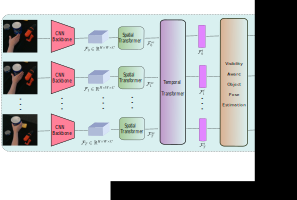
\includegraphics[width=0.98\linewidth]{figs/overview}
	\caption{Overview of the proposed framework for in-hand object pose tracking. Our approach leverages transformers to capture both spatial relationships within individual frames and temporal dependencies across image sequences, enabling robust frame-wise object pose estimation. To address challenges posed by heavy occlusion or motion blur, a visibility-aware module integrates temporally-aware features and aggregates pose information from neighboring frames. This allows the model to maintain accurate pose estimates even in difficult scenarios where direct visual cues are limited or absent.}
	\label{fig:overview}
\end{figure*}

The overview structure of our framework is illustrated in Figure \ref{fig:overview}. Given a sequence of RGB images $\mathcal{V} = \lbrace I_t \rbrace_{t=1}^{T}$, where $T$ represents the total number of frames, the objective is to estimate the object's 6D pose $\mathbf{P}_t = (\mathbf{R}_t, \mathbf{t}_t)$ for each frame $I_t$. This pose consists of the rotation matrix $\mathbf{R}_t$ and the translation vector $\mathbf{t}_t$, which describe the rigid transformation of the object from its coordinate system to the camera coordinate system. We assume that a 3D model of the object is available, and its coordinate system is defined within the 3D space of the model. The framework first utilizes a CNN backbone to extract spatial features \( \mathcal{F}_t \) from each frame. These features are then enhanced by a spatial transformer $\mathcal{M}_{s}$, which captures non-local dependencies within each frame to improve the modeling of complex hand-object interactions. The spatial transformer encoder produces contextually enriched features \( \mathcal{F}^s_t \), which are further processed by a temporal transformer $\mathcal{M}_{s}$ that models temporal relationships across frames. The temporal transformer outputs latent vectors \( \mathcal{F}^t_t \), which are passed through an MLP to predict the object's pose \( \hat{\mathbf{P}}_t \) for each frame. Additionally, a visibility-aware module $\mathcal{M}_{va}$ predicts the object's visibility score \( v_t \) for each frame, dynamically adjusting pose predictions based on occlusion levels. This module aggregates pose information from visible frames to support pose estimation in occluded frames using a cross-attention mechanism, ensuring robust performance under heavy occlusions and rapid motion.

\subsection{Spatial-Temporal Transformer}

\subsubsection{CNN Backbone}

Inspired by the hybrid model proposed by \cite{carion2020end}, our method begins by leveraging a truncated FPN \cite{lin2017feature} with ResNet50 \cite{he2016deep} to extract the initial in-hand object features $\mathcal{F}_t \in \mathbb{R}^{H \times W \times C}$ for each frame $I_t$. While CNNs, through their convolutional kernels, are effective at capturing local two-dimensional structures, they struggle with occlusions where local details are obscured or distorted. To mitigate this, we incorporate a transformer \cite{vaswani2017attention}, which is adept at handling non-local relationships and dependencies. The feature maps $\mathcal{F}_t$ are subsequently processed by a spatial transformer, which captures non-local dependencies within each frame, enhancing the network's ability to model complex interactions between the object and the hand.

\subsubsection{Spatial Transformer}

The spatial transformer encoder processes a sequence as input. To facilitate this, we flatten the spatial dimensions of the hand feature, resulting in $HW$ vectors, each with length $C$. These vectors, referred to as tokens, are then fed through multiple layers of multi-head self-attention and feed-forward networks (FFN). Since each transformer layer is permutation-invariant, we incorporate 2D positional embeddings into each token to provide spatial location information. The output feature $\mathcal{F}^s_t \in \mathbb{R}^{H \times W \times C}$ from the transformer encoder enhances the original feature $\mathcal{F}_t$ by capturing non-local interactions among all tokens. This enhanced feature $\mathcal{F}^s_t$ is expected to contain rich contextual information about the in-hand object, including the locations of object keypoints. We follow previous works \cite{oberweger2018making, tekin2018real, rad2017bb8} use the eight corners of the 3D bounding box of the object as the keypoints. As an intermediate supervision step, we regress a heatmap of object keypoint joints $\hat{\mathcal{H}}_t$ from $\mathcal{F}^s_t$, which provides the predicted locations of $N_j = 8$ keypoints as $\hat{\mathcal{K}} \in \mathbb{R}^{8 \times 2}$.

The spatial transformer decoder takes a learnable query vector $\mathbf{Q} \in \mathbb{R}^C$ as input and progressively integrates information from the combined features of $\mathcal{F}^s_t$ and $\hat{\mathcal{K}}$ through several layers of cross-attention and FFN. Unlike self-attention, which generates query, key, and value from the same set of tokens, cross-attention uses the learnable query vector to create the query and leverages the learned tokens for key and value. Following  \cite{jaegle2021perceiver}, the decoder adaptively selects relevant information from the feature map, producing a compact latent representation $\mathcal{F}^{se}_t \in \mathbb{R}^C$ of the object. This significantly reduces the computational cost for temporal reasoning in subsequent stages.

\subsubsection{Temporal Transformer}

Relying solely on single images for hand-held object pose estimation is often insufficient due to several challenges. One issue is the variability in the object's visual appearance over time, which can lead to inconsistent predictions from image-based models. Additionally, the object is frequently occluded by the hand or itself during interaction, making it difficult to estimate its pose accurately when only a portion of the object is visible. Videos, however, offer the advantage of capturing different views and movements of the object, which can reveal parts that might be occluded or blurred in a single frame. This advantage motivates the use of a transformer encoder to model feature interactions along the temporal dimension. Unlike traditional recurrent architectures that process frames sequentially, the transformer's self-attention mechanism allows each frame to leverage information from all other frames directly, regardless of their position in the sequence \cite{vaswani2017attention}. This approach enables the model to capture long-range temporal dependencies more effectively. Similar to the spatial transformer encoder, the temporal transformer encoder processes the sequence of features $\lbrace\mathcal{F}^{se}_t\rbrace_{t=1}^{T}$, which are enhanced by the spatial transformer, and outputs a new set of latent vectors $\lbrace\mathcal{F}^{t}_t\rbrace_{t=1}^{T}$. Given $\mathcal{F}^t_t$, an MLP (Multi-Layer Perceptron) serves as the pose regression network, processing these features to predict the initial object pose parameters $\hat{\mathbf{P}}_t$. By incorporating information across multiple frames, the model can more accurately predict the object's pose, even in cases where individual frames are challenging to interpret due to rapid motion. 

\subsection{\DIFdelbegin \DIFdel{Visibility-aware }\DIFdelend \DIFaddbegin \DIFadd{Visibility-Aware }\DIFaddend Object Pose Estimation \DIFdelbegin \DIFdel{under occlusions}\DIFdelend \DIFaddbegin \DIFadd{Under Occlusions}\DIFaddend }

Our \DIFdelbegin \DIFdel{network with }\DIFdelend \DIFaddbegin \DIFadd{proposed framework leverages }\DIFaddend spatial and temporal transformers \DIFdelbegin \DIFdel{recovers more accurate object pose }\DIFdelend \DIFaddbegin \DIFadd{to improve object pose estimation accuracy}\DIFaddend . However, \DIFdelbegin \DIFdel{the object pose prediction under very heavy occlusions remains challenging because no image evidence from single frameis available for accurate prediction. Our key idea is to use the }\DIFdelend \DIFaddbegin \DIFadd{predicting object poses under heavy occlusion remains particularly challenging due to the lack of sufficient image evidence within a single frame. To address this issue, we propose a novel approach that combines }\DIFaddend temporally-aware features\DIFaddbegin \DIFadd{, }\DIFaddend $\mathcal{F}^t_t$\DIFdelbegin \DIFdel{of }\DIFdelend \DIFaddbegin \DIFadd{, from the }\DIFaddend current occluded frame \DIFdelbegin \DIFdel{and object pose }\DIFdelend \DIFaddbegin \DIFadd{with object pose information }\DIFaddend from other visible frames to predict the \DIFdelbegin \DIFdel{object of occluded frames. To this end, we first predict object visibility scores in each image}\DIFdelend \DIFaddbegin \DIFadd{pose of the occluded object. This is achieved by first estimating visibility scores for each frame}\DIFaddend , which are \DIFdelbegin \DIFdel{then leveraged together with the object evidence from neighbouring frames to predict the object poses of the occluded }\DIFdelend \DIFaddbegin \DIFadd{subsequently used to guide the aggregation of pose evidence from neighboring visible }\DIFaddend frames.

\subsubsection{Visibility Estimation\DIFdelbegin \DIFdel{.}\DIFdelend }

We introduce a visibility score $v_t \in [0, 1]$ for each frame $t$, \DIFdelbegin \DIFdel{representing the extent to which the object is visible}\DIFdelend \DIFaddbegin \DIFadd{which quantifies the visibility of the object in that frame}\DIFaddend . This score is crucial for identifying \DIFdelbegin \DIFdel{frames where the object is heavily occluded by the hand or other objects}\DIFdelend \DIFaddbegin \DIFadd{heavily occluded frames where direct pose estimation is unreliable}\DIFaddend . The visibility score is predicted using a visibility decoder $f_{vis}(\cdot)$, which operates on \DIFdelbegin \DIFdel{the }\DIFdelend temporally-aware features $\mathcal{F}^t_t$. The \DIFdelbegin \DIFdel{visibility }\DIFdelend decoder consists of \DIFdelbegin \DIFdel{a series of }\DIFdelend fully connected layers\DIFdelbegin \DIFdel{that map the high-dimensional features $\mathcal{F}^t_t$ to a scalar visibility score. The final layer applies }\DIFdelend \DIFaddbegin \DIFadd{, culminating in }\DIFaddend a sigmoid activation function to ensure \DIFdelbegin \DIFdel{that the score lies }\DIFdelend \DIFaddbegin \DIFadd{outputs lie }\DIFaddend within the range $[0, 1]$:

\begin{equation}
v_t = \sigma(f_{vis}(\mathcal{F}^t_t)),
\end{equation}

\noindent where $\sigma(\cdot)$ denotes the sigmoid function. The visibility score $v_t$ \DIFdelbegin \DIFdel{effectively captures }\DIFdelend \DIFaddbegin \DIFadd{represents }\DIFaddend the confidence level of \DIFdelbegin \DIFdel{the object being visible }\DIFdelend \DIFaddbegin \DIFadd{object visibility }\DIFaddend in frame $t$. For \DIFdelbegin \DIFdel{each }\DIFdelend \DIFaddbegin \DIFadd{training, the ground truth visibility score $v_t$ is computed as the fraction of visible object pixels in }\DIFaddend frame $t$\DIFdelbegin \DIFdel{in the dataset, let }\DIFdelend \DIFaddbegin \DIFadd{, defined as:
}

\begin{equation}
\DIFadd{v_t = \frac{|O_t|}{|O|},
}\end{equation}

\noindent \DIFadd{where }\DIFaddend $O$ \DIFdelbegin \DIFdel{represent the set of all }\DIFdelend \DIFaddbegin \DIFadd{is the total set of }\DIFaddend annotated object pixels, and \DIFdelbegin \DIFdel{let }\DIFdelend $O_t$ \DIFdelbegin \DIFdel{represent }\DIFdelend \DIFaddbegin \DIFadd{represents }\DIFaddend the subset of \DIFdelbegin \DIFdel{those pixels that remain }\DIFdelend \DIFaddbegin \DIFadd{pixels }\DIFaddend visible in frame $t$. The \DIFdelbegin \DIFdel{ground truth visibility score $v_t$ is computed as:
}%DIFDELCMD < 

%DIFDELCMD < %%%
\begin{displaymath}
\DIFdel{v_t = \frac{|O_t|}{|O|}.
}\end{displaymath}
%DIFAUXCMD
%DIFDELCMD < 

%DIFDELCMD < \noindent %%%
\DIFdel{To train the }\DIFdelend visibility estimation network \DIFdelbegin \DIFdel{, we define a loss function that measures the difference between the predicted visibility score $v_t$ and the ground truth visibility score $v_t$. We use }\DIFdelend \DIFaddbegin \DIFadd{is trained using }\DIFaddend the Binary Cross Entropy (BCE) loss\DIFdelbegin \DIFdel{function, which is commonly used for binary classification tasks and is suitable for training models to output values in the range $[0, 1]$. The BCE loss for the visibility estimation can be expressed as}\DIFdelend \DIFaddbegin \DIFadd{, which measures the difference between predicted visibility scores $\hat{v}_t$ and ground truth scores $v_t$}\DIFaddend :

\begin{equation}
\mathcal{L}_{vis} = - \frac{1}{N} \sum_{t=1}^{N} \left( v_t \log(\hat{v}_t) + (1 - v_t) \log(1 - \hat{v}_t) \right),
\end{equation}

\noindent where \DIFdelbegin \DIFdel{:
}%DIFDELCMD < \begin{itemize}
%DIFDELCMD <     \item %%%
\DIFdelend $N$ is the total number of frames in the dataset. \DIFdelbegin %DIFDELCMD < \item %%%
\DIFdel{$\hat{v}_t$ is the predicted visibility score for frame $t$.
    }%DIFDELCMD < \item %%%
\DIFdel{$v_t$ is the ground truth visibility score for frame $t$.
    }%DIFDELCMD < \item %%%
\DIFdel{The terms $v_t \log(\hat{v}_t)$ and $(1 - v_t) \log(1 - \hat{v}_t)$ penalize the model for incorrect predictions by comparing the predicted scores against the ground truth.
}%DIFDELCMD < \end{itemize}
%DIFDELCMD < %%%
\DIFdelend \DIFaddbegin \DIFadd{This loss function penalizes incorrect predictions while ensuring the model outputs confidence values that align with ground truth visibility.
}\DIFaddend 

\subsubsection{Object Pose Prediction Under Heavy Occlusion\DIFdelbegin \DIFdel{.}\DIFdelend }

\DIFdelbegin \DIFdel{Our objective is to accurately predict the object pose for frames where the object is heavily occluded (i.e., frames with a visibility score \( v_i \) smaller than \( \delta = 0.5 \)) . We achieve this by employing a Pose Transformer that aggregates temporal information from frames where the object is visible . This aggregated pose information is then combined with the feature vector of the occluded frame to recover the object's pose. For clarity, we will refer to the temporally-aware features of the occluded frames\( \mathcal{F}_t^t \) as \( \mathcal{F}_{occ} \)}\DIFdelend \DIFaddbegin \DIFadd{Accurate object pose prediction for heavily occluded frames (visibility score $v_i < \delta$}\DIFaddend , where \DIFdelbegin \DIFdel{\( \mathcal{F}_{occ} \in \mathbb{R}^C \). }%DIFDELCMD < 

%DIFDELCMD < \noindent %%%
\DIFdelend \DIFaddbegin \DIFadd{$\delta = 0.5$) is achieved by aggregating temporal pose information from visible frames. }\DIFaddend The Pose Transformer \DIFdelbegin \DIFdel{aggregates temporal pose information }\DIFdelend \DIFaddbegin \DIFadd{is used to integrate pose embeddings }\DIFaddend from multiple visible frames, \DIFdelbegin \DIFdel{leveraging the consistency across these frames to improve pose estimation under occlusion. Let \(\hat{\mathbf{P}}_t \) represent the pose of the object at time \( t \), where \( t \) corresponds to the visible frames. These poses are first }\DIFdelend \DIFaddbegin \DIFadd{ensuring consistent pose estimation even under occlusions. Temporally-aware features from occluded frames, $\mathcal{F}^t_t$, are denoted as $\mathcal{F}_{occ} \in \mathbb{R}^C$.
}

\DIFadd{To aggregate pose information, visible-frame poses $\hat{\mathbf{P}}_t$ are }\DIFaddend embedded into a \DIFdelbegin \DIFdel{higher-dimensional space, forming pose embeddings \( \mathbf{E}_t \in \mathbb{R}^d \), where \( d \) is the dimensionality of the embedding space. These pose embeddings from multiple visible frames, \( \{\mathbf{E}_{t_1}, \mathbf{E}_{t_2}, \dots, \mathbf{E}_{t_n}\} \), are used as input to }\DIFdelend \DIFaddbegin \DIFadd{high-dimensional space, resulting in pose embeddings $\mathbf{E}_t \in \mathbb{R}^d$. These embeddings are processed by }\DIFaddend the Pose Transformer\DIFdelbegin \DIFdel{. The transformer employs }\DIFdelend \DIFaddbegin \DIFadd{, which uses }\DIFaddend a multi-head self-attention mechanism \DIFdelbegin \DIFdel{, which computes attention scores \( \alpha_{ij} \) between each pair of pose embeddings\( \mathbf{E}_i \) and \( \mathbf{E}_j \) across the visible frames. These attention scores are computed using the equation
}\DIFdelend \DIFaddbegin \DIFadd{to compute attention scores $\alpha_{ij}$ between embeddings:
}\DIFaddend 

\begin{equation}
\alpha_{ij} = \DIFdelbegin \DIFdel{softmax}\DIFdelend \DIFaddbegin \DIFadd{\text{softmax}}\DIFaddend \left(\frac{\mathbf{Q}_i \cdot \mathbf{K}_j^T}{\sqrt{d_k}}\right),
\end{equation}

\noindent where \DIFdelbegin \DIFdel{\( \mathbf{Q}_i = \mathbf{E}_i \mathbf{W}_Q \) and \( \mathbf{K}_j = \mathbf{E}_j \mathbf{W}_K \) are the queryand keyvectors obtained by projecting the pose embeddings }\DIFdelend \DIFaddbegin \DIFadd{$\mathbf{Q}_i = \mathbf{E}_i \mathbf{W}_Q$, $\mathbf{K}_j = \mathbf{E}_j \mathbf{W}_K$, and $\mathbf{V}_j = \mathbf{E}_j \mathbf{W}_V$ are query, key, and value vectors, respectively. These are obtained }\DIFaddend using learnable weight matrices \DIFdelbegin \DIFdel{\( \mathbf{W}_Q \in \mathbb{R}^{d \times d_k} \) }\DIFdelend \DIFaddbegin \DIFadd{$\mathbf{W}_Q, \mathbf{W}_K, \mathbf{W}_V \in \mathbb{R}^{d \times d_k}$, }\DIFaddend and \DIFdelbegin \DIFdel{\( \mathbf{W}_K \in \mathbb{R}^{d \times d_k} \), with \( d_k \) typically set to \( \frac{d}{num\_heads} \), where \( num\_heads \) is the number of attention heads. The value vectors \( \mathbf{V}_j = \mathbf{E}_j \mathbf{W}_V \) are obtained through another projection matrix \( \mathbf{W}_V \in \mathbb{R}^{d \times d_v} \).
The output of the transformer is the }\DIFdelend \DIFaddbegin \DIFadd{$d_k = d / \text{num\_heads}$.
}

\DIFadd{The transformer outputs an }\DIFaddend aggregated pose feature \DIFdelbegin \DIFdel{\( \mathbf{Z}_{agg} \in \mathbb{R}^d \)}\DIFdelend \DIFaddbegin \DIFadd{$\mathbf{Z}_{agg} \in \mathbb{R}^d$}\DIFaddend , which integrates temporal information from the visible frames. \DIFdelbegin \DIFdel{Once the aggregated pose feature \( \mathbf{Z}_{agg} \) is obtained from the Pose Transformer, it }\DIFdelend \DIFaddbegin \DIFadd{This feature }\DIFaddend is combined with the \DIFdelbegin \DIFdel{feature vector \( \mathcal{F}_{occ} \in \mathbb{R}^C \) of the occluded frame. The feature vector \( \mathcal{F}_{occ} \) is extracted from the temporal transformer, which processes the }\DIFdelend occluded frame's \DIFdelbegin \DIFdel{visual data. To combine these features, }\DIFdelend \DIFaddbegin \DIFadd{feature vector $\mathcal{F}_{occ}$ through }\DIFaddend a cross-attention mechanism\DIFdelbegin \DIFdel{is employed, where the aggregated pose feature \( \mathbf{Z}_{agg} \) }\DIFdelend \DIFaddbegin \DIFadd{, where $\mathbf{Z}_{agg}$ }\DIFaddend serves as the query \DIFdelbegin \DIFdel{, and the occluded frame's feature vector \( \mathcal{F}_{occ} \) }\DIFdelend \DIFaddbegin \DIFadd{and $\mathcal{F}_{occ}$ }\DIFaddend provides the keys and values. Specifically, the query \DIFdelbegin \DIFdel{vector isgenerated by projecting the aggregated pose feature}\DIFdelend \DIFaddbegin \DIFadd{is}\DIFaddend :

\begin{equation}
\mathbf{Q}_{agg} = \mathbf{Z}_{agg} \mathbf{W}_Q' \in \mathbb{R}^{d_q},
\end{equation}

\noindent \DIFdelbegin \DIFdel{where \( \mathbf{W}_Q' \in \mathbb{R}^{d \times d_q} \) is a learnable weight matrix, and \( d_q \) is the dimensionality of the query vector. The }\DIFdelend \DIFaddbegin \DIFadd{while }\DIFaddend keys and values are obtained \DIFdelbegin \DIFdel{by projecting the feature vector \( \mathcal{F}_{occ} \)}\DIFdelend \DIFaddbegin \DIFadd{as}\DIFaddend :

\begin{equation}
\mathbf{K}_{occ} = \mathcal{F}_{occ} \mathbf{W}_K' \in \mathbb{R}^{d_k},
\end{equation}

\begin{equation}
\mathbf{V}_{occ} = \mathcal{F}_{occ} \mathbf{W}_V' \in \mathbb{R}^{d_v}\DIFdelbegin \DIFdel{,
}\DIFdelend \DIFaddbegin \DIFadd{.
}\DIFaddend \end{equation}

\noindent \DIFdelbegin \DIFdel{where \( \mathbf{W}_K' \in \mathbb{R}^{C \times d_k} \) and \( \mathbf{W}_V' \in \mathbb{R}^{C \times d_v} \) are learnable weight matrices for the keys and values, respectively. The query \( \mathbf{Q}_{agg} \) then attends to the keys \( \mathbf{K}_{occ} \) to compute the attention weights }\DIFdelend \DIFaddbegin \DIFadd{The cross-attention weights are computed as}\DIFaddend :

\begin{equation}
\beta_{ij} = \DIFdelbegin \DIFdel{softmax}\DIFdelend \DIFaddbegin \DIFadd{\text{softmax}}\DIFaddend \left(\frac{\mathbf{Q}_{agg} \cdot \mathbf{K}_{occ}^T}{\sqrt{d_k}}\right),
\end{equation}

\noindent \DIFdelbegin \DIFdel{where \( \mathbf{K}_{occ} \) is the key vector from the occluded frame's feature vector. The final }\DIFdelend \DIFaddbegin \DIFadd{resulting in the }\DIFaddend fused feature representation\DIFdelbegin \DIFdel{is computed as a weighted sum of the value vectors}\DIFdelend :

\begin{equation}
\mathcal{F}_{fused} = \sum_{j=1}^{C} \beta_{ij} \mathbf{V}_{occ}\DIFdelbegin \DIFdel{\in \mathbb{R}^{d_v}}\DIFdelend .
\end{equation}

\noindent \DIFdelbegin \DIFdel{This cross-attention mechanism allows the aggregated pose feature to dynamically interact with the occluded frame's feature vector, guiding the network to focus on the most relevant information for pose estimation. The output \( \mathcal{F}_{fused} \) effectively integrates temporal pose information from the visible frames with the features of the occluded frame, providing a robust foundation for accurate pose prediction under heavy occlusion. Given the enhanced feature, we use an MLPto estimate the final pose parameter }\DIFdelend \DIFaddbegin \DIFadd{The fused feature $\mathcal{F}_{fused}$ integrates information from both visible and occluded frames, enabling accurate pose predictions under occlusion. Finally, a multi-layer perceptron (MLP) processes $\mathcal{F}_{fused}$ to predict the object's pose }\DIFaddend $\hat{\mathbf{P}}_{occ}$ for \DIFdelbegin \DIFdel{occluded frames}\DIFdelend \DIFaddbegin \DIFadd{the occluded frame. This approach ensures that the temporal information from visible frames compensates for the lack of visual evidence in heavily occluded frames, resulting in robust and accurate pose estimation}\DIFaddend .

\subsection{Loss Function}

For asymmetric objects, the loss function is defined as the average Euclidean distance between the model points transformed by the ground truth pose and the predicted pose:

\begin{equation}
\mathcal{L}_{pose} = \frac{1}{N} \sum_{i=1}^{N} \left\| (\mathbf{R} \mathbf{x}_i + \mathbf{t}) - (\hat{\mathbf{R}} \mathbf{x}_i + \hat{\mathbf{t}}) \right\|_2,
\end{equation}

\noindent where:

\begin{itemize}
    \item $\mathbf{R}$ and $\mathbf{t}$ are the ground truth rotation matrix and translation vector.
    \item $\hat{\mathbf{R}}$ and $\hat{\mathbf{t}}$ are the predicted rotation matrix and translation vector.
    \item $\mathbf{x}_i$ represents the $i$-th point in the object's model.
    \item $N$ is the total number of points sampled on the object model.
    \item $\left\| \cdot \right\|_2$ is the Euclidean norm, measuring the distance between the two sets of transformed points.
\end{itemize}

\noindent For symmetric objects, the above loss function is not well-defined due to the potential for multiple canonical frames. Instead, we use a modified loss function that minimizes the distance between each point on the estimated model orientation and the closest point on the ground truth model:

\begin{equation}
\mathcal{L}_{pose} = \frac{1}{N} \sum_{i=1}^{N} \min_{j} \left\| (\mathbf{R} \mathbf{x}_j + \mathbf{t}) - (\hat{\mathbf{R}} \mathbf{x}_i + \hat{\mathbf{t}}) \right\|_2.
\end{equation}

\noindent In addition to the pose loss, we introduce a keypoint-based loss function. Keypoints are defined as distinctive points on the object that are consistent across frames. The keypoint loss is computed as the average Euclidean distance between the predicted keypoints $\hat{\mathbf{k}}_i$ and the ground truth keypoints $\mathbf{k}_i$:

\begin{equation}
\mathcal{L}_{keypoint} = \frac{1}{M} \sum_{i=1}^{M} \left\| \mathbf{k}_i - \hat{\mathbf{k}}_i \right\|_2,
\end{equation}

\noindent where:

\begin{itemize}
    \item $\mathbf{k}_i$ represents the $i$-th ground truth keypoint.
    \item $\hat{\mathbf{k}}_i$ is the corresponding predicted keypoint.
    \item $M$ is the total number of keypoints.
\end{itemize}

\noindent The total loss function now combines the pose estimation loss, the keypoint loss, and the visibility-aware loss:

\begin{equation}
\mathcal{L}_{total} = \mathcal{L}_{pose} + \lambda_{key} \mathcal{L}_{keypoint} + \lambda_{vis} \mathcal{L}_{vis},
\end{equation}

\noindent where $\lambda_{key}$ and $\lambda_{vis}$ are weights that balance the contribution of the keypoint loss and the visibility-aware loss in the total loss function.

%
\input{diff_Results}
%
\bibliographystyle{IEEEtran}
\bibliography{References}

\begin{IEEEbiography}[{\includegraphics[width=1in,height=1.25in,clip,keepaspectratio]{authors/prof_Tan}}]{Phan Xuan Tan} (Member, IEEE) received the B.E. degree in Electrical-Electronic Engineering from Military Technical Academy, Vietnam, M.E. degree in Computer and Communication Engineering from Hanoi University of Science and Technology, Vietnam and Ph.D. degree in Functional Control Systems from Shibaura Institute of Technology, Japan. He is currently an Associate Professor at Shibaura Institute of Technology. His current research interests include computer vision, deep learning and image processing.
\end{IEEEbiography}

\begin{IEEEbiography}[{\includegraphics[width=1in,height=1.25in,clip,keepaspectratio]{authors/DinhCuong}}]{Dinh-Cuong Hoang} received his Ph.D. degree in computer science from Orebro University, Sweden (2021), and is currently a lecturer at FPT University, Greenwich Vietnam. His research interests lie at the intersection of computer vision, robotics, and machine learning. He is particularly interested in topics involving autonomy for robots, with a focus on perception algorithms.
\end{IEEEbiography}

\begin{IEEEbiography}[{\includegraphics[width=1in,height=1.25in,clip,keepaspectratio]{authors/Eiji_Kamioka}}]{Eiji Kamioka} (Member, IEEE) received the B.S., M.S., and D.S. degrees in physics from Aoyama Gakuin University. He is a Professor with the Shibaura Institute of Technology (SIT). Before joining the SIT, he was working with the SHARP Communication Laboratory, Institute of Space and Astronautical Science (ISAS), as a JPSP Research Fellow, and the National Institute of Informatics (NII) as an Assistant Professor. His current research interests encompass mobile multimedia communications and ubiquitous computing.
\end{IEEEbiography}

\begin{IEEEbiography}[{\includegraphics[width=1in,height=1.25in,clip,keepaspectratio]{authors/NguyenAnhNhat}}]{Anh-Nhat Nguyen}  is currently a lecturer at FPT University, Vietnam. He received his B.S. and M.S. degrees in Computer Science from Duy Tan University, Da Nang, Vietnam, in 2012 and from Huazhong University of Science and Technology (HUST), China, in 2018, respectively. His research interests include image processing, information security, physical layer secrecy, radio-frequency energy harvesting, and wireless sensor networks.
\end{IEEEbiography}

\begin{IEEEbiography}[{\includegraphics[width=1in,height=1.25in,clip,keepaspectratio]{authors/TranDucThanh}}]{Duc-Thanh Tran} is pursuing a B.S. degree in Artificial Intelligence at FPT University, Hanoi, Vietnam, with a primary focus on research in the field of computer vision.
\end{IEEEbiography}

\begin{IEEEbiography}[{\includegraphics[width=1in,height=1.25in,clip,keepaspectratio]{authors/DuongVanHiep}}]{Van-Hiep Duong} is pursuing a B.S. degree in Artificial Intelligence at FPT University, Hanoi, Vietnam, with a primary focus on research in the field of computer vision.
\end{IEEEbiography}

\begin{IEEEbiography}[{\includegraphics[width=1in,height=1.25in,clip,keepaspectratio]{authors/MaiAnhTruong}}]{Anh-Truong Mai} is pursuing a B.S. degree in Artificial Intelligence at FPT University, Hanoi, Vietnam, with a primary focus on research in the field of computer vision.
\end{IEEEbiography}

\begin{IEEEbiography}[{\includegraphics[width=1in,height=1.25in,clip,keepaspectratio]{authors/PhamDucLong}}]{Duc-Long Pham} is pursuing a B.S. degree in Artificial Intelligence at FPT University, Hanoi, Vietnam, with a primary focus on research in the field of computer vision.
\end{IEEEbiography}

\begin{IEEEbiography}[{\includegraphics[width=1in,height=1.25in,clip,keepaspectratio]{authors/PhanKhanhToan}}]{Khanh-Toan Phan} is pursuing a B.S. degree in Artificial Intelligence at FPT University, Hanoi, Vietnam, with a primary focus on research in the field of computer vision.
\end{IEEEbiography}

\begin{IEEEbiography}[{\includegraphics[width=1in,height=1.25in,clip,keepaspectratio]{authors/DuongVanHiep}}]{Van-Hiep Duong} is pursuing a B.S. degree in Artificial Intelligence at FPT University, Hanoi, Vietnam, with a primary focus on research in the field of computer vision.
\end{IEEEbiography}

\begin{IEEEbiography}[{\includegraphics[width=1in,height=1.25in,clip,keepaspectratio]{authors/DinhXuanTung}}]{Xuan-Tung Dinh} is pursuing a B.S. degree in Artificial Intelligence at FPT University, Hanoi, Vietnam, with a primary focus on research in the field of computer vision.
\end{IEEEbiography}

\begin{IEEEbiography}[{\includegraphics[width=1in,height=1.25in,clip,keepaspectratio]{authors/TranThiThuyTrang}}]{TranThiThuyTrang} is pursuing a B.S. degree in Information Technology at FPT University, Hanoi, Vietnam.
\end{IEEEbiography}

\begin{IEEEbiography}[{\includegraphics[width=1in,height=1.25in,clip,keepaspectratio]{authors/PhamXuanDuong}}]{Xuan-Duong Pham} is pursuing a B.S. degree in Information Technology at FPT University, Hanoi, Vietnam.
\end{IEEEbiography}

\begin{IEEEbiography}[{\includegraphics[width=1in,height=1.25in,clip,keepaspectratio]{authors/NguyenNhatLinh}}]{Nhat-Linh Nguyen} is pursuing a B.S. degree in Information Technology at FPT University, Hanoi, Vietnam.
\end{IEEEbiography}

\begin{IEEEbiography}[{\includegraphics[width=1in,height=1.25in,clip,keepaspectratio]{authors/ThuUyenNguyen}}]{Thu-Uyen Nguyen} is pursuing a B.S. degree in Artificial Intelligence at FPT University, Hanoi, Vietnam, with a primary focus on research in the field of computer vision.
\end{IEEEbiography}

\begin{IEEEbiography}[{\includegraphics[width=1in,height=1.25in,clip,keepaspectratio]{authors/TrinhVietAnh}}]{Viet-Anh Trinh} is pursuing a B.S. degree in Information Technology at Greenwich Vietnam, FPT University, Hanoi, Vietnam.
\end{IEEEbiography}

\begin{IEEEbiography}[{\includegraphics[width=1in,height=1.25in,clip,keepaspectratio]{authors/TranKhanhDuong}}]{Khanh-Duong Tran} is pursuing a B.S. degree in Information Technology at Greenwich Vietnam, FPT University, Hanoi, Vietnam.
\end{IEEEbiography}

\begin{IEEEbiography}[{\includegraphics[width=1in,height=1.25in,clip,keepaspectratio]{authors/BuiSonAnh}}]{Son-Anh Bui} is pursuing a B.S. degree in Information Technology at Greenwich Vietnam, FPT University, Hanoi, Vietnam.
\end{IEEEbiography}

\EOD

\end{document}
